\chapter{QUIC Protocol}\label{chap:02-quic}

This chapter is intended as a summary of the QUIC protocol specification providing sufficient detail
for our implementation design. The text is based on version 29 of the draft specification documents
from June 2020, more specifically on the documents describing the core transport
protocol~\cite{draft-ietf-quic-transport}, TLS integration~\cite{draft-ietf-quic-tls}, and
congestion control mechanism~\cite{draft-ietf-quic-recovery}. Readers familiar with these documents
may skip this chapter.

We will start this chapter by first providing a high-level overview of QUIC and then providing a
more detailed description of the protocol's individual parts.

\section{Overview of QUIC}

QUIC protocol provides reliable and secure transport of multiple streams of data over a single
connection\footnote{The ability to transport multiple streams over a single connection is called
\textit{stream multiplexing}}. QUIC is implemented on top of UDP, which provides only unreliable
transfer of datagrams. In addition to stream multiplexing, QUIC also implements loss recovery,
congestion control, transport security, and other features known from TCP or TLS protocols.

\subsection{QUIC Connection}

As in other protocols, QUIC allows communication between two endpoints: client and server. In QUIC
connection, endpoints exchange QUIC packets. A single UDP datagram can contain multiple packets,
although it generally contains only one. Bundling multiple QUIC packets in a single UDP datagram is
called \textit{coalescing}. QUIC packets cannot span multiple UDP datagrams.

In order to identify QUIC connections, endpoints use Connection IDs negotiated during connection
establishment. Each endpoint independently chooses a Connection ID it will use to identify the
connection. When sending a QUIC packet, the endpoint uses these Connection IDs to populate the
\textit{Source Connection ID} (SCID for short) and \textit{Destination Connection ID} (DCID for
short) fields of the QUIC packet header.

\todo{list all abbreviations at the end/beginning of the thesis?}.

\todo{ remove the stuff about socket multiplexing? The socket multiplexing stuff is not mentioned in the spec, nor it is the expected usage scenario. }

The separation of connection identity from the used socket allows multiple connections to be made
using the same socket. \autoref{fig:02-connection-multiplexing} illustrates how the incoming packets
are associated with individual connections based on the DCID field of the packet header.

\begin{myFigure}{fig:02-connection-multiplexing}{Multiple QUIC connections on the same machine port}

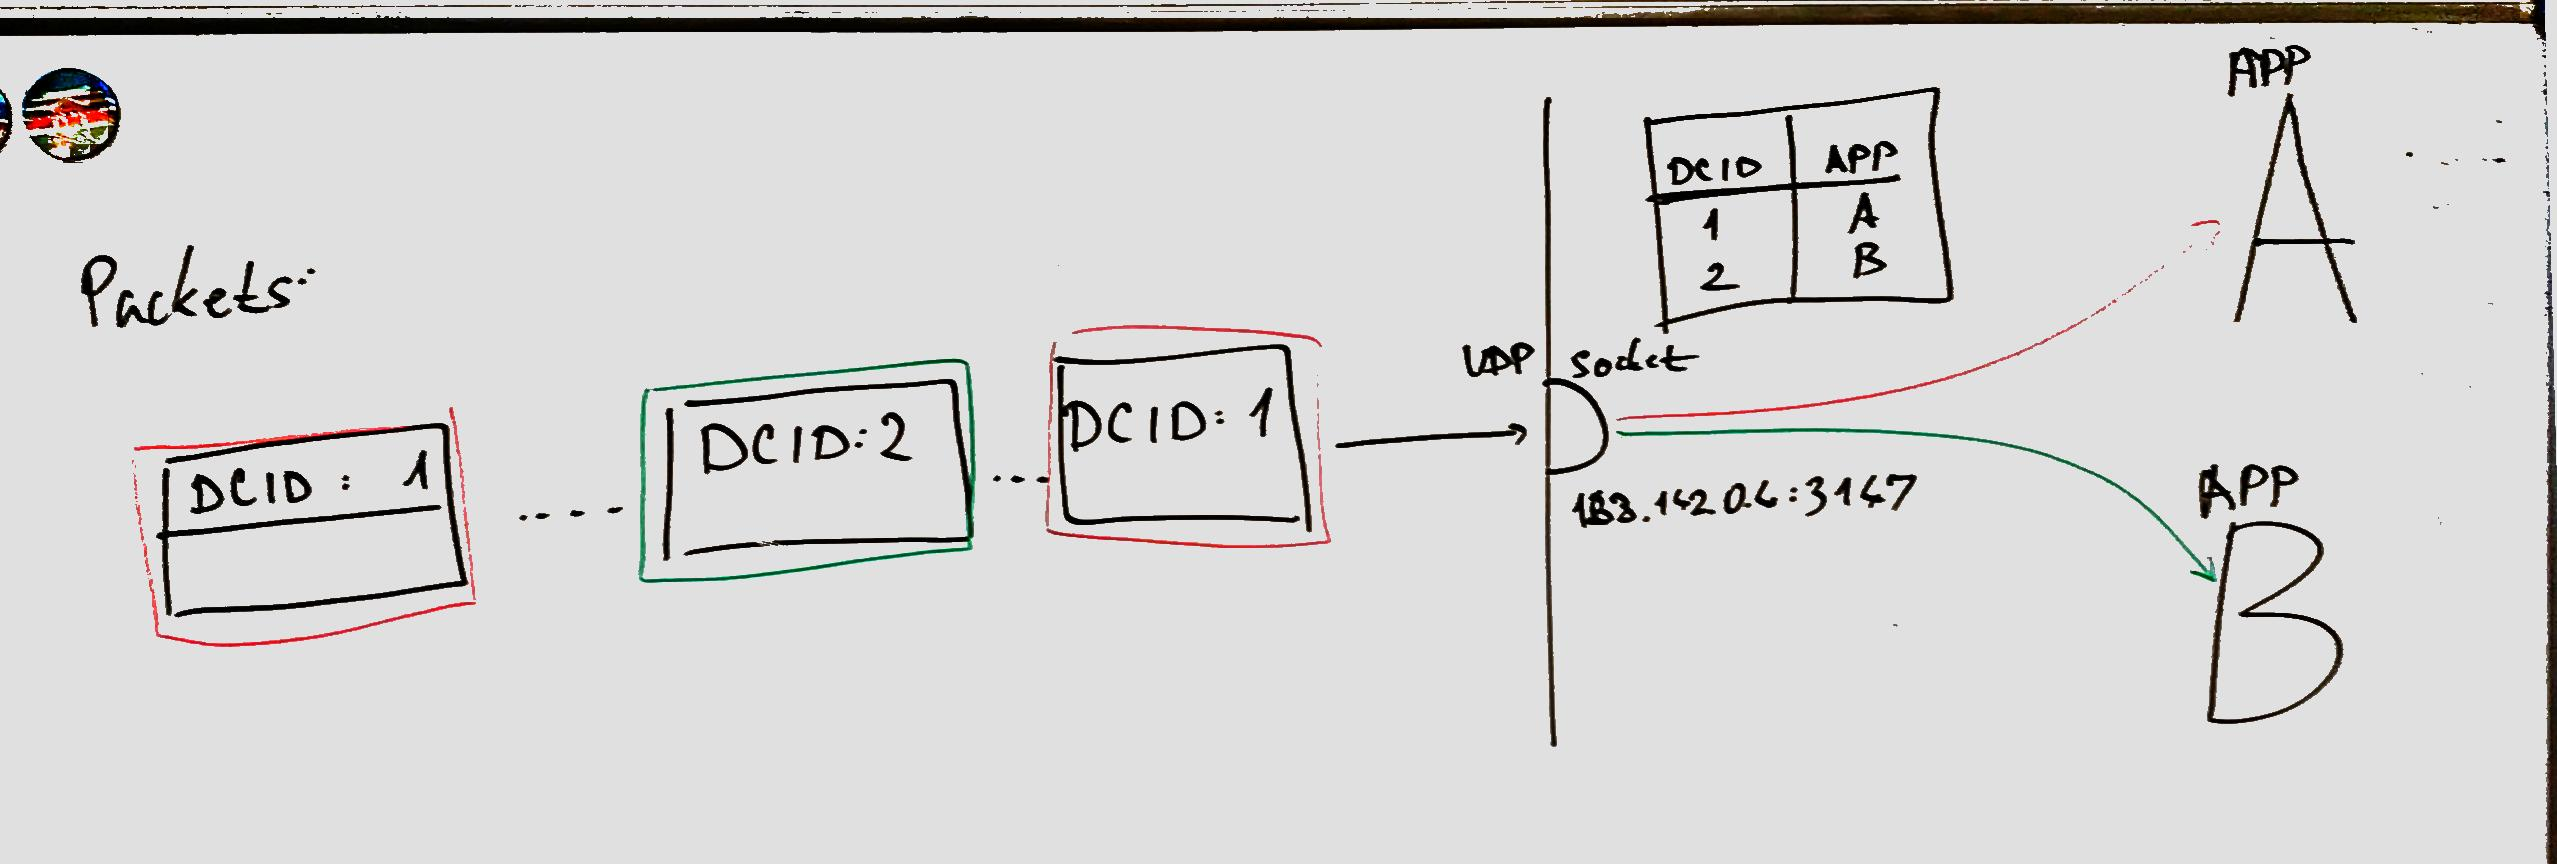
\includegraphics[width=0.9\textwidth]{img/02-socket-multiplexing}

\end{myFigure}

\todo{better describe the image, it is hard to decipher, TODO, really different applications?}

\subsection{QUIC Packets}

QUIC packets sent in the UDP datagram are the smallest processible unit of QUIC\@. The packets are
formed by a header and a variable-length payload consisting of one or more QUIC frames. QUIC frames
carry individual pieces of information, such as acknowledgments or stream data sent by the
application.

Similarly to TCP, packets in QUIC connections are numbered. However, QUIC uses three separate
\textit{Packet number spaces}:

\begin{enumerate}

  \litem{Initial} Used for exchanging initial information.

  \litem{Handshake} Used during the connection handshake process.

  \litem{1-RTT} Used throughout the lifetime of the connection to transfer application data.

\end{enumerate}

Packets from each packet number space are numbered and processed independently of the other packet
spaces. This also includes acknowledgments for received packets. An acknowledgment for an Initial
packet can be sent only in another Initial packet and vice versa.

\subsection{Packet Encryption}

QUIC uses symmetric cryptographic ciphers to encrypt QUIC packets. Each packet number space uses
different keys for packet encryption. Keys for the Initial packet number space are derived using
only the client's Connection ID and therefore provide obfuscation rather than protection. Handshake
keys are intermediate protection keys derived by the TLS protocol during the TLS handshake. 1-RTT
keys are negotiated by the TLS 1.3 protocol and offer the same security level as in a standard TLS
1.3 connection. QUIC uses packet encryption to protect both against network traffic observers and
packet payload corruption.

\subsection{Stream Multiplexing}

QUIC can transport multiple streams of data in a single connection. Each stream can be either
unidirectional or bidirectional and is identified by its Stream ID. Each stream is processed
independently of the other streams. \autoref{fig:02-stream-multiplexing} illustrates how QUIC may
pack two streams into frames such that those streams are transported in parallel.

\begin{myFigure}{fig:02-stream-multiplexing}{Stream multiplexing in QUIC}

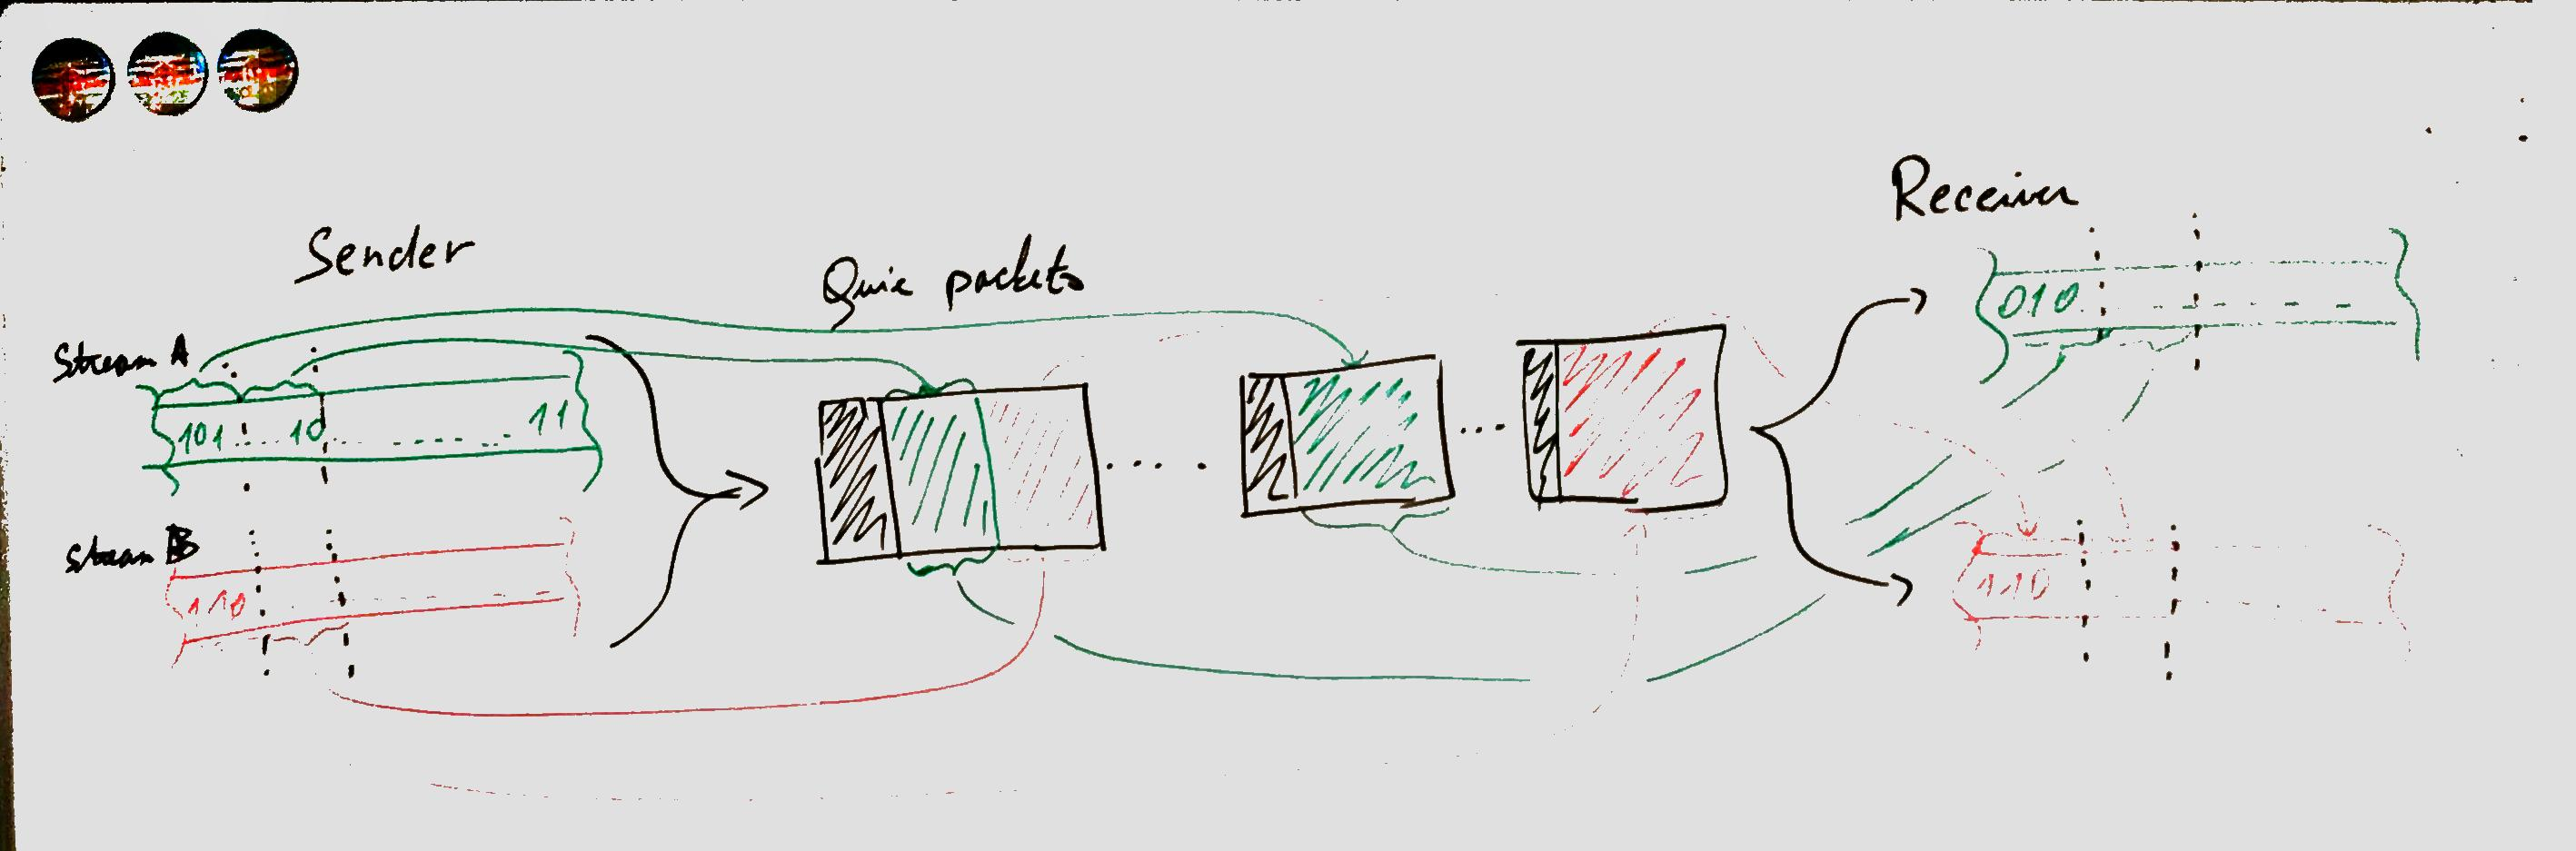
\includegraphics[width=0.9\textwidth]{img/02-stream-multiplexing}

\end{myFigure}

\todo{change the picture so that the newest data is on the right side, basically, just flip the
stream on the Sender's side}

\subsection{Flow Control}

As a prevention against malicious too fast senders, QUIC implements a credit-based flow-control
scheme. Each endpoint advertises how much data it is willing to accept and how many streams of each
type can be opened by its peer.

\subsection{Loss Detection and Recovery}

Because UDP is an unreliable transport protocol, QUIC must implement measures to recover from packet
loss. The packet loss detection is implemented similarly to TPC. Each endpoint sends acknowledgments
for each received packet. However, an essential difference from TCP is that QUIC endpoints do not
retransmit lost packets with the same packet numbers. Instead, each QUIC frame in the original
packet is updated and sent in some future packet or dropped altogether if it is no longer relevant.

\autoref{fig:02-packet-loss-example} illustrates the retransmission process. When the sender
receives the acknowledgment for packet 3, it infers that packet 2 never reached the receiver, and
retransmits the STREAM frame in packet 4. The sender does not have to retransmit the ACK for packet
1 because it was already sent in packet 3. Therefore, packet 4 includes ACK only for packet 2.

\todo{redraw the image to match the description above}

\begin{myFigure}{fig:02-packet-loss-example}{Retransmission of lost data in QUIC}

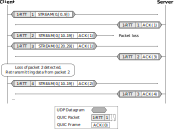
\includegraphics[width=0.5\textwidth]{img/02-retransmission-example}

\end{myFigure}

\todo{Also, make the image more like a UML process diagram}

\subsection{Wire Encoding}

The process of encoding QUIC packets to be sent via the network is optimized for size. All values
sent over the network are encoded in Big-Endian, also known as \textit{network order}. Almost all
numerical values are encoded using a variable-length integer encoding. This encoding uses the first
byte's two most significant bits to encode whether the value is encoded as 1, 2, 4, or 8-byte
integer. This encoding supports only positive numbers. The ranges available for individual encoding
lengths are listed in \autoref{tab:02-quic-varint-length}.

\begin{myTable} {tab:02-quic-varint-length} {Variable-length integer encoding lengths}
  {ccr}
  {Most significant bits & Encoding length (B) & Maximum value}
  00                     & 1                   & \num{63}         \\
  01                     & 2                   & \num{16383}      \\
  10                     & 4                   & \num{1073741824} \\
  11                     & 8                   & $2^{62}-1$       \\
\end{myTable}

In order to optimize the size of QUIC packets, the implementations are encouraged to always choose
the shortest encoding necessary to represent the given number.

\section{QUIC Connection}

In the overview section, we mentioned that QUIC endpoints use Connection IDs to identify connections
and that they exchange UDP datagrams with QUIC packets containing QUIC frames.

\subsection{Connection ID}

The primary function of a connection ID is to ensure that changes in addressing at lower protocol
layers (UDP, IP) do not cause packets for a QUIC connection to be delivered to the wrong endpoint.

Endpoints in the connection select Connection IDs for the other endpoint to use when sending
packets. There can be more than one Connection ID identifying the connection for the endpoint.
During the connection lifetime, each endpoint can issue additional Connection IDs, or retire
connection IDs issued by the other endpoint.

By retiring a Connection ID, the endpoint communicates that it will no longer use the Connection ID,
and the other endpoint should drop any incoming packets that use it. Retiring a Connection ID serves
as a request to the peer to issue a new Connection ID as a replacement.

Each Connection ID is bound to local and destination addresses. During connection migration, the
endpoints must start using different Connection ID to prevent correlation of the network traffic.

\subsection{QUIC Packets}

QUIC uses a total of five different packet types:

\begin{enumerate}

  \litem{Initial \textnormal{and} Handshake} used during connection establishment;

  \litem{1-RTT} main packets used during the lifetime of QUIC connection;

  \litem{Version Negotiation} sent by the server when the client tries to establish a connection
  using an unsupported version of QUIC\@;

  \litem{0-RTT} carries \textit{early data} when TLS 1.3 0-RTT mode of operation is enabled; and

  \litem{Retry} optionally used by servers for client's address validation when establishing new
  connections.

\end{enumerate}

Packets of type Initial, Handshake, and 1-RTT correspond to the packets sent in the connection's
three packet number spaces. For packet processing purposes like acknowledgments and loss detection,
the 1-RTT packet number space also includes 0-RTT packets.

Version Negotiation and Retry packets are used in special cases. They are not associated with a
packet number space and are neither numbered nor encrypted.

Packets of different types contain different fields. The packet types can be separated into two
groups: packets with so called \textit{long header}, and packets with \textit{short header}. The
form of the header determines the fields in the header, with short header containing fewer fields to
improve efficiency of the protocol. All packets except 1-RTT packets use the long header format.

The following list explains the meaning of the individual packet fields. The list also indicates if
the field is specific to a particular header or packet type.

\newcommand\ditemLh[1]{\ditemWithComment{#1}{long header only}}
\newcommand\ditemSh[1]{\ditemWithComment{#1}{short header only}}

\begin{description}

    \ditem{Header Form Bit} used to distinguish between packets with so called \textit{long header}
    and \textit{short header} format

    \ditem{Fixed Bit}  A bit that is always set to 1 in valid packets.

    \ditemLh{Long Packet Type} Discriminator of the packet type.

    \ditemLh{Version} Indicates which version of QUIC is in use and determines how rest of the
    protocol fields are interpreted.

    \ditemLh{Destination Connection ID Length} Length of the Destination Connection ID.

    \ditem{Destination Connection ID}  The Connection ID issued by the recipient of the packet.

    \ditemLh{Source Connection ID Length}  Length of the Source Connection ID.

    \ditemLh{Source Connection ID} The Connection ID issued by the sender of the packet. Note that
    1-RTT packets do not contain this field because the sender is authenticated by the encryption.

    \ditem{Reserved Bits} Bits reserved for use in the next QUIC versions. In the initial QUIC
    version, these bits are set to 0.

    \ditemWithComment{Packet Number Length}{Initial, Handshake, 1-RTT, 0-RTT packets}
    The length of the encoding used for the packet number. The packet number does not use the
    variable-length encoding. Instead, the packet number is truncated and up to 4 least significant
    bytes are included in the packet. The length of the truncated packet number is always chosen so
    that the other endpoint can safely reconstruct the full packet number.

    \ditemWithComment{Length}{Initial, Handshake, 1-RTT, 0-RTT packets} The length of the remainder
    of the packet. This includes the Packet Number, the payload of the packet, and --- for encrypted
    packets --- the AEAD integrity tag.

    \ditemWithComment{Packet Number}{Initial, Handshake, 1-RTT, 0-RTT packets} The truncated packet
    number.

    \ditemSh{Spin Bit} A bit used for optional on-path latency measurements.

    \ditemWithComment{Retry Token}{Initial, Retry packets} Contains an opaque token generated by the server to validate the clients address.

    \ditemWithComment{Retry Integrity Tag}{Retry packet only} A tag used by servers during client
    address validation during connection establishment.

    \ditemSh{Key Phase Bit} A bit used to communicate an encryption key update.

\end{description}

\subsection{QUIC Frames}

Packets of type Initial, Handshake, 0-RTT and 1-RTT packets carry low-level QUIC protocol messages
called QUIC frames. These include, e.g., ACK frames carrying acknowledgments for received packets,
STREAM frames carrying application data, and CRYPTO frames carrying data for TLS handshake.

Even though all received QUIC packets have to be acknowledged, some packets do not need to be
acknowledged immediately. For example, packets containing only ACK frames are not acknowledged
immediately to avoid unnecessary network traffic. Instead, the acknowledgment is sent later together
with other data. Frame types requiring immediate acknowledgments are called \textit{ack-eliciting
frames}, and the packets with at least one such frame are called \textit{ack-eliciting packets}.

There are multiple restrictions on which frames can be sent in which packets. For example, STREAM
frames can only be sent in 1-RTT packets to avoid compromising security.
\autoref{tab:02-frame-types} lists all frame types, whether they are ack-eliciting and in which
packets they can be sent.

\begin{myTable}[\small] {tab:02-frame-types} {QUIC frame types}
  {l@{\hskip -0.1in}ccccc}
  {                      &               & \multicolumn{4}{c}{Allowed in packet type}                \\ \cmidrule(lr){3-6}
    Frame type           & Ack-eliciting & Initial      & Handshake    & 0-RTT        & 1-RTT}
  PADDING                &               & \checkmark{} & \checkmark{} & \checkmark{} & \checkmark{} \\
  PING                   & \checkmark{}  & \checkmark{} & \checkmark{} & \checkmark{} & \checkmark{} \\
  ACK                    &               & \checkmark{} & \checkmark{} &              & \checkmark{} \\
  RESET\_STREAM          & \checkmark{}  &              &              & \checkmark{} & \checkmark{} \\
  STOP\_SENDING          & \checkmark{}  &              &              & \checkmark{} & \checkmark{} \\
  CRYPTO                 & \checkmark{}  & \checkmark{} & \checkmark{} &              & \checkmark{} \\
  NEW\_TOKEN             & \checkmark{}  &              &              &              & \checkmark{} \\
  STREAM                 & \checkmark{}  &              &              & \checkmark{} & \checkmark{} \\
  MAX\_DATA              & \checkmark{}  &              &              & \checkmark{} & \checkmark{} \\
  MAX\_STREAM\_DATA      & \checkmark{}  &              &              & \checkmark{} & \checkmark{} \\
  MAX\_STREAMS           & \checkmark{}  &              &              & \checkmark{} & \checkmark{} \\
  DATA\_BLOCKED          & \checkmark{}  &              &              & \checkmark{} & \checkmark{} \\
  STREAM\_DATA\_BLOCKED  & \checkmark{}  &              &              & \checkmark{} & \checkmark{} \\
  STREAMS\_BLOCKED       & \checkmark{}  &              &              & \checkmark{} & \checkmark{} \\
  NEW\_CONNECTION\_ID    & \checkmark{}  &              &              & \checkmark{} & \checkmark{} \\
  RETIRE\_CONNECTION\_ID & \checkmark{}  &              &              & \checkmark{} & \checkmark{} \\
  PATH\_CHALLENGE        & \checkmark{}  &              &              & \checkmark{} & \checkmark{} \\
  PATH\_RESPONSE         & \checkmark{}  &              &              & \checkmark{} & \checkmark{} \\
  CONNECTION\_CLOSE      &               & \checkmark{} & \checkmark{} & \checkmark{} & \checkmark{} \\
  HANDSHAKE\_DONE        & \checkmark{}  &              &              &              & \checkmark{} \\
\end{myTable}

\subsection{Connection Establishment}

A QUIC connection is considered established when the TLS handshake completes. By then, both peers
have derived the necessary protection keys and can receive 1-RTT frames with application data.

An example handshake flow is illustrated in \autoref{fig:02-example-handshake-flow}. The figure also
lists the contents of the CRYPTO frames sent. However, this is only for illustrative purposes
because QUIC does not interpret the CRYPTO frames' contents.

\begin{myFigure} {fig:02-example-handshake-flow} {Example QUIC handshake flow}

\begin{verbatim}
   Client                                                  Server

   Initial[0]: CRYPTO[CH] ->

                                    Initial[0]: CRYPTO[SH] ACK[0]
                          Handshake[0]: CRYPTO[EE, CERT, CV, FIN]
                                    <- 1-RTT[0]: STREAM[1, "..."]

   Initial[1]: ACK[0]
   Handshake[0]: CRYPTO[FIN], ACK[0]
   1-RTT[0]: STREAM[0, "..."], ACK[0] ->

                                             Handshake[1]: ACK[0]
                            <- 1-RTT[1]: STREAM[3, "..."], ACK[0]
\end{verbatim}

  \todo{Note that this is copied from RFC? Also, this example lacks the
    HANDSHAKE\_DONE frame}

  \todo{Make this diagram graphical, not textual}
\end{myFigure}

In its first datagram, the client sends an Initial packet with a single CRYPTO frame containing the
\textit{Client Hello} TLS message.

The server replies with a datagram containing three coalesced QUIC packets. The first is an Initial
packet that acknowledges the client's Initial packet, and a CRYPTO frame with a \textit{Server
Hello} message. The contents of Client Hello and Server Hello messages are used by TLS to derive
Handshake protection keys. The server advances the TLS handshake further by sending another CRYPTO
frame in the Handshake packet. The server also has enough information to derive also the 1-RTT keys,
so it can also start sending data on Stream 1 using the STREAM frame in a 1-RTT packet.

Because the server's Initial packet contained an ack-eliciting CRYPTO frame, the client needs to
respond with another Initial frame with an ACK frame. The client can now derive the Handshake keys,
enabling him to process the server's Handshake packet. The Handshake packet needs to be separately
acknowledged by an ACK frame, and a reply from the TLS layer must be sent using another CRYPTO
frame. From the information in the server's Handshake packet's CRYPTO frame, the client derives
1-RTT protection keys and processes the server's 1-RTT packet. In addition to sending an ACK frame
for the server's 1-RTT packet, the client can now start sending application data on stream 0 using a
STREAM frame.

\subsection{Connection Termination}

QUIC connection can be terminated in three ways:

\begin{itemize}

  \item Idle timeout

  \item Immediate close

  \item Stateless reset

\end{itemize}

\subsubsection{Idle Timeout}\label{sec:idle-timeout}

If idle timeout is enabled, the endpoint silently closes the connection if it does not receive a
packet from the peer for a specified time period. Each peer may advertise a timeout period using the
\texttt{max\_idle\_timeout} transport parameter, but the effective value is the minimum of the two
values.

In order to prevent timeouts, endpoints can send a PING or another ack-eliciting frame to test the
liveness of the connection. However, sending PING frames should be initiated by the application
protocol, not QUIC implementation, to prevent unnecessary network traffic.

\subsubsection{Immediate close}

An immediate close can be initiated both by QUIC implementation and by the application protocol.
Either endpoint can initiate an immediate close by sending a CONNECTION\_CLOSE frame. This causes
all streams to become closed immediately.

By sending a CONNECTION\_CLOSE frame, the peer enters a closing state, in which it includes the
CONNECTION\_CLOSE frame in all packets it sends in reply to incoming packets.

Upon receiving a CONNECTION\_CLOSE, the peer should echo the CONNECTION\_CLOSE back to the peer and
enter the closing state.

The closing state lasts until the endpoint is sure the other endpoint is also in the closing state
(e.g., until it also receives CONNECTION\_CLOSE), or until a closing timeout expires. The closing
timeout period is calculated from the current estimate of the round-trip time of the connection.

The CONNECTION\_CLOSE frame carries an error code and, optionally, a human-readable error phrase.
When initiated by QUIC, the error codes semantics defined by the QUIC specification. However, when
initiated by the application protocol, the semantics of all possible error code values sent in the
frame are defined by the application protocol itself.

\subsubsection{Stateless reset}

A stateless reset is an option of last resort for an endpoint that does not have access to the state
of a connection, possibly resulting from a crash or outage. An endpoint may send a stateless reset
in response to receiving a packet that it cannot associate with an active connection.

In such cases, the endpoint sends a specially crafted packet that ends with a Stateless Reset Token
associated with his Connection ID\@. The Stateless Reset Token requirements are quite complex, and
we encourage readers to read the full specification if they are interested in details. \todo{include
reference to the appropriate section?}

\subsection{TLS Extensions used by QUIC}

QUIC uses some of the standard TLS extensions. The first is Application Level Protocol
Negotiation~\cite{rfc7301} (ALPN for short). When multiple application protocols are supported on
the same TCP or UDP port, ALPN allows the application layer to negotiate --- as part of the TLS
handshake --- which protocol will be used.

The second TLS extension used is Server Name Indication~\cite{rfc6066} (SNI for short). Clients use
this extension to specify the hostname of the server to which they are connecting. When multiple
websites are hosted on the same IP address and port, SNI allows the server to use the SSL
certificate and other security configuration for the website requested by the client.

\subsection{QUIC Transport Parameters}

QUIC leverages the extensibility of the TLS handshake to also exchange specific parameters for the
connections. Many of the parameters have a default value, which is used when the given transport
parameter is not sent. However, some transport parameters are mandatory in some cases. Example
information set through transport parameters is:

\begin{itemize}

  \item Initial flow control limits

  \item Whether connection migration is allowed

  \item Maximum delay before sending an acknowledgment for ack-eliciting packets

  \item Maximum idle timeout before the connection is silently closed

  \item Maximum size of a UDP packet the endpoint is willing to receive

\end{itemize}

\section{Streams}

Streams transported by QUIC can be either unidirectional or bidirectional. Unidirectional streams
carry data from the initiator to its peer, and bidirectional streams carry data in both directions.
Both client and server can open new streams. QUIC recognizes four types of streams, and the type of
the stream is encoded in the two least significant bits of the Stream ID. The stream types and their
associated encoding is summarized in \autoref{tab:02-stream-id-type-map}.

\begin{myTable} {tab:02-stream-id-type-map} {Mapping of QUIC Stream types to Stream ID bits}
  {cc}
  {Stream type                     & Least significant bits}
  Client-Initiated, Bidirectional  & 00 \\
  Server-Initiated, Bidirectional  & 01 \\
  Client-Initiated, Unidirectional & 10 \\
  Server-Initiated, Unidirectional & 11 \\
\end{myTable}

For example, client-initiated unidirectional streams have Stream IDs 2, 6, 10, and so on. The Stream
ID is encoded using the variable-length integer encoding and, therefore, can range from 0 to
$2^{62}-1$. However, endpoints must use the next lowest Stream ID for the given stream type when
opening a new stream.

Bidirectional streams can be viewed as the combination of two unidirectional streams. After opening
the stream, each direction of the stream behaves as separate inbound and outbound unidirectional
streams. This means, e.g., that the reading and writing part of the stream can be closed
independently of each other.

Streams are opened simply by sending the first STREAM frame for that stream. The endpoint sending
data on the stream can close the stream either gracefully by specifying that all data have been
written or by abruptly terminating the stream using RESET\_STREAM frame. The abrupt termination is
also referred to as \textit{resetting the stream}. The endpoint receiving the stream can request a
stream reset using the STOP\_SENDING frame if it no longer wishes to receive data on that stream.
Abrupt termination of the stream requires specifying an application-level error code that is
communicated to the peer.

Implementations should provide a way for application protocols to specify the relative priority of
streams.

The implementation should provide the following operations on sending part of the stream:

\begin{itemize}

  \item write data;

  \item end the stream by specifying that all data has been written; and

  \item terminate the stream with an application-level error code.

\end{itemize}

On receiving part of the stream, application protocols need to be able to:

\begin{itemize}

  \item read data; and

  \item abort reading with an application-level error code.

\end{itemize}

\section{Flow Control}

QUIC aims to be a general-purpose transport protocol to be used over a potentially untrusted
network, and as such, it needs to protect endpoints from malicious peers. To prevent malicious
senders from exhausting all available memory on the receiver by sending large amounts of data, or
fast senders from overwhelming slow receivers, QUIC employs a credit-based flow control scheme.

All QUIC streams are flow controlled both individually and together as an aggregate. Each endpoint
also controls the number of streams the other peer is allowed to open. All flow control limits are
communicated to the peer using three types of frames:

\begin{itemize}

\litem{MAX\_STREAM\_DATA} maximum offset of data sent on a stream with specified ID\@.

\litem{MAX\_DATA} maximum sum of all offsets of data sent on all streams.

\litem{MAX\_STREAMS} maximum number of opened streams of a particular stream type.

\end{itemize}

Endpoints can only increase the flow control limits. Their peers must ignore any attempts to
decrease the flow control limits to ensure consistency when two consecutive QUIC packets with flow
control updates are reordered during transit.

In case the peer violates any of the control flow limits mentioned above, the QUIC implementation
must immediately terminate the connection.

\section{Loss Detection and Recovery}

To ensure that the peer receives sent data, QUIC requires each endpoint to send acknowledgments for
all packets using ACK frames. The ACK frames contain ranges of packet numbers that the endpoint
acknowledges.

QUIC declares a packet lost when it meets the following conditions:

\begin{enumerate}

  \item The packet was not is unacknowledged.

  \item A packet sent later has been acknowledged.

  \item Either the packet has been sent long enough in the past, or its packet number is
sufficiently smaller than any acknowledged packet sent later.

\end{enumerate}

The third condition is dependent on the values of particular constants. The specification recommends
that the packet is considered lost if the gap between its packet number and the next acknowledged
packet is at least 3, or if it was sent for longer than $9/8$ times the estimate of the current
round-trip time.

The first condition mentioned above requires receipt of a packet from the peer to declare any packet
as lost. However, the loss of the last packet in a sequence could go undetected because no following
packet to be acknowledged has been sent. To avoid possible deadlocks in such scenarios, QUIC
endpoint sens a \textit{probe packet} if it does not receive a packet from a peer in a period called
\textit{probe timeout} (PTO for short). QUIC endpoints send up to 2 probe packets. The PTO duration
doubles each time probe packets are sent until either a reply is received or the connection is
terminated due to idle timeout (see \autoref{sec:idle-timeout})

Similarly to TCP, QUIC also uses congestion control to manage the \textit{congestion window} --- the
amount of data that can be in-flight. The QUIC-RECOVERY specification document describes a
congestion control algorithm similar to TCP NewReno~\cite{rfc6582} algorithm. However, it leaves the
selection of the congestion control algorithm up to the implementation.

\section{Packet Protection}

All QUIC packets of type Initial, Handshake, 1-RTT and 0-RTT are encrypted to ensure integrity and
confidentiality of the transmitted data. Negotiation of the cryptographic ciphers and the encryption
keys is handled by the TLS handshake. This section focuses on how the negotiated encryption is
applied to QUIC packets.

\subsection{Authenticated Encryption with Associated Data}

QUIC uses type of encryption called Authenticated encryption with associated data~\cite{rfc5116}
(AEAD for short). This type of encryption ensures both confidentiality and authenticity of the
encrypted data. In addition to encrypted data, AEAD encryption outputs also an authentication tag
which is used to check the integrity of the payload during decryption. The encryption can be
authenticated by supplying additional authentication data (AAD for short) which are not encrypted,
but influence the authentication tag and, therefore, must be supplied also during decryption. As an
additional protection, AEAD also accepts a \textit{nonce} parameter, which is an additional input
which is supposed to be unique for each encrypted packet.

The programming interface for AEAD provides following operations:

\begin{itemize}

  \item Encryption:

  \begin{itemize}

    \item input: plaintext, key, nonce, AAD (optional)

    \item output: ciphertext, authentication tag

  \end{itemize}

  \item Decryption:

  \begin{itemize}

    \item input: ciphertext, key, nonce, authentication tag, AAD (if provided during encryption)

    \item output: plaintext or error if the authentication tag does not match the supplied
      ciphertext and AAD

  \end{itemize}

\end{itemize}

\subsection{Deriving QUIC Protection Keys}

QUIC derives multiple distinct keys from the secrets negotiated by TLS handshake. The derivation
uses the HKDF-Expand-Label function~\cite{rfc5869} to derive keys of desired length. The keys are
derived as follows:

\begin{equation*}
  \begin{split}
  key & = \operatorname{HKDF-Expand-Label}(secret, \texttt{"quic key"}, \texttt{""}, 32) \\
  iv  & = \operatorname{HKDF-Expand-Label}(secret, \texttt{"quic iv"}, \texttt{""}, 12)  \\
  hp  & = \operatorname{HKDF-Expand-Label}(secret, \texttt{"quic hp"}, \texttt{""}, 32)  \\
  \end{split}
\end{equation*}

The following subsections describe how the $key$, $iv$, and $hp$ keys are used in the actual process
of packet encryption.

\subsection{Packet Protection Procedure}

When actually encrypting the packets, QUIC first encrypts the packet payload using the AEAD cipher
negotiated by the TLS implementation. The parameters for AEAD are:

\begin{itemize}

    \litem{key} the $key$ derived in previous section

    \litem{nonce} the $iv$ derived in previous section, last 8 bytes XORed with the packet number

    \litem{AAD} the contents of the packet header

    \litem{plaintext} the payload of the packet.

\end{itemize}

The produced authentication tag is appended to the protected payload and is included in the payload
size.

QUIC also protects the header of the packet. The header protection mechanism is more complex than
that of the payload. The process requires calculating the \textit{header protection mask}, which is
then applied using exclusive OR to parts of the packet header. The details of the header protection
mask calculation depend on the negotiated cipher, but it always uses the $hp$ key and a 16-byte
sample of the encrypted payload.

\todo{Try illustrating the process using a figure}

\subsection{Updating 1-RTT Protection Keys}

Some AEAD functions have limits for how many packets can be encrypted using the same keys. Analysis
in the specification document shows that updating the protection keys after sending at most
$2^{23}$ packets provides the same confidentiality level as a standard TLS connection~\cite{draft-ietf-quic-tls}.

The key update is signalled by flipping a \textit{key phase} bit in the 1-RTT packet header. And
after observing the change in the \textit{key phase}, an endpoint derives new secret and $key$ and
$iv$ keys using the HKDF-Expand-Label function:

\begin{equation*}
  \begin{split}
  secret_{n+1} & = \operatorname{HKDF-Expand-Label}(secret_{n}, \texttt{"quic ku"}, \texttt{""}, 32) \\
  key_{n+1} & = \operatorname{HKDF-Expand-Label}(secret_{n+1}, \texttt{"quic key"}, \texttt{""}, 32) \\
  iv_{n+1}  & = \operatorname{HKDF-Expand-Label}(secret_{n+1}, \texttt{"quic iv"}, \texttt{""}, 12)  \\
  \end{split}
\end{equation*}

Because the \textit{key phase} bit is protected by header protection, the $hp$ key must remain
unchanged to ensure that the other endpoint can correctly remove the header protection.

\section{Additional Features}

\subsection{Peer validation?}

\subsection{Connection migration}
